% MH1812 — Chapter 4: Proof (0->100 ground-up)
\chapter[Proof]{Proof: Direct, Contrapositive, Contradiction and Induction}
\label{ch:proof}

\begin{quote}
\emph{``A proof is a story that convinces even a sceptical reader.''} We systematise four story patterns that cover almost every theorem in discrete mathematics.
\end{quote}

\noindent\fbox{\parbox{\dimexpr\linewidth-2\fboxsep-2\fboxrule}{%
\textbf{From zero: proving from scratch.} We move from ``why should I believe it?'' to formal templates: assume premise $\to$ deduce conclusion (direct), flip to contrapositive, seek a clash (contradiction), and climb an infinite ladder (induction \& strong induction).}}
\vspace{0.4em}

\section*{Learning Outcomes}
After this chapter you will be able to:
\begin{enumerate}[label=(L\arabic*)]
    \item structure direct proofs from definitions;
    \item prove $P\to Q$ via its contrapositive $\neg Q\to\neg P$;
    \item use contradiction to prove negations and impossibility;
    \item prove universal statements over $\mathbb{N}$ by weak and strong induction;
    \item spot faulty induction and fix base cases and inductive hypotheses.
\end{enumerate}

% ============================================================
\section{Direct Proof}
\label{sec:direct}
To prove $P\to Q$, assume $P$ and derive $Q$ using definitions, algebra, and prior theorems. Start by writing what $P$ and $Q$ mean.

\begin{definition}[Even and odd]
$n\in\mathbb{Z}$ is \emph{even} if $n=2k$ for some $k\in\mathbb{Z}$; \emph{odd} if $n=2k+1$.
\end{definition}

\begin{example}[Direct]
Claim: If $n$ is odd then $n^2$ is odd. Proof: $n=2k+1\Rightarrow n^2=4k^2+4k+1=2(2k^2+2k)+1$, odd. \qed
\end{example}

\begin{example}[Direct with divisibility]
Claim: If $a\mid b$ and $b\mid c$ then $a\mid c$. Proof: $b=ak$, $c=b\ell=ak\ell$, so $a\mid c$.
\end{example}

\begin{theorem}[Sum of two rationals is rational]
If $x,y\in\mathbb{Q}$ then $x+y\in\mathbb{Q}$.
\end{theorem}
\begin{proof} Write $x=p/q$, $y=r/s$ with integers, $q,s\neq0$; then $x+y=(ps+rq)/qs\in\mathbb{Q}$.
\end{proof}

\begin{figure}[h]\centering
\begin{tikzpicture}[scale=0.82,every node/.style={font=\scriptsize}]
% Proof strategy flowchart with colors
\node[draw,thick,rounded corners=3pt,fill=blue!14,minimum width=3.2cm,minimum height=0.9cm,align=center] (goal) at (0,3) {Goal: prove $P\to Q$};
\node[draw,thick,diamond,fill=green!14,aspect=2,align=center,inner sep=2pt] (dec) at (0,1.5) {What form\\is $Q$?};
\node[draw,thick,rounded corners=3pt,fill=orange!16,minimum width=3.0cm,minimum height=0.9cm,align=center] (direct) at (-3.8,0) {Direct:\\assume $P$, derive $Q$};
\node[draw,thick,rounded corners=3pt,fill=violet!14,minimum width=3.0cm,minimum height=0.9cm,align=center] (contra) at (0,0) {Contrapositive:\\assume $\neg Q$, derive $\neg P$};
\node[draw,thick,rounded corners=3pt,fill=red!14,minimum width=3.0cm,minimum height=0.9cm,align=center] (contrad) at (3.8,0) {Contradiction:\\assume $P\land\neg Q$,\\derive $R\land\neg R$};
\node[draw,thick,rounded corners=3pt,fill=yellow!18,minimum width=3.0cm,minimum height=0.9cm,align=center] (ind) at (0,-1.5) {Induction:\\$P(n)$ for all $n\ge n_0$};
\draw[->,thick,blue!60!black] (goal)--(dec);
\draw[->,thick,blue!60!black] (dec)--(direct) node[midway,above,sloped,font=\tiny] {$Q$ positive};
\draw[->,thick,blue!60!black] (dec)--(contra) node[midway,right,font=\tiny] {$Q=\neg R$};
\draw[->,thick,blue!60!black] (dec)--(contrad) node[midway,above,sloped,font=\tiny] {no easier form};
\draw[->,thick,blue!60!black] (dec)--(ind) node[midway,right,font=\tiny] {$\forall n$};
\node[font=\tiny,fill=gray!10,rounded corners=2pt,inner sep=2pt] at (0,-2.5) {Choose the cheapest path that fits the goal's shape.};
\end{tikzpicture}
\caption{Choosing a proof strategy by inspecting the goal. Colour helps memorise: green decision, warm options.}
\label{fig:proof-strategy}
\end{figure}

\section{Contrapositive}
\label{sec:contrapositive}
$P\to Q\equiv\neg Q\to\neg P$. When $Q$ is a negation or $P$ messy, proving $\neg Q\to\neg P$ is cleaner --- yet still a direct proof of the flipped statement.

\begin{example}
Claim: If $n^2$ is even then $n$ is even. Direct is awkward (square root). Contrapositive: if $n$ odd ($n=2k+1$) then $n^2$ odd (proved above). \qed
\end{example}

\begin{lemma}
If $x^2$ irrational implies $x$ irrational? Contrapositive: rational $x=p/q\Rightarrow x^2=p^2/q^2$ rational.
\end{lemma}

\section{Contradiction}
\label{sec:contradiction}
To prove $P$, assume $\neg P$ and derive $R\land\neg R$.

\begin{theorem}[Irrationality of $\sqrt2$]
$\sqrt2\notin\mathbb{Q}$.
\end{theorem}
\begin{proof} Assume $\sqrt2=p/q$ in lowest terms, $\gcd(p,q)=1$, $q>0$. Then $2q^2=p^2\Rightarrow p$ even $=2k\Rightarrow 2q^2=4k^2\Rightarrow q^2=2k^2\Rightarrow q$ even --- both even contradicts $\gcd=1$.
\end{proof}

\begin{theorem}[Infinitely many primes]
There are infinitely many primes.
\end{theorem}
\begin{proof} Suppose $p_1,\dots,p_k$ were all primes. Let $N=p_1\cdots p_k+1$. $N$ has a prime divisor $p$ (proved by induction). $p$ cannot be any $p_i$ (remainder $1$), contradiction.
\end{proof}

\section{Induction and Strong Induction}
\label{sec:induction}
Induction is dominoes: knock first, each knocks next.

\begin{figure}[h]\centering
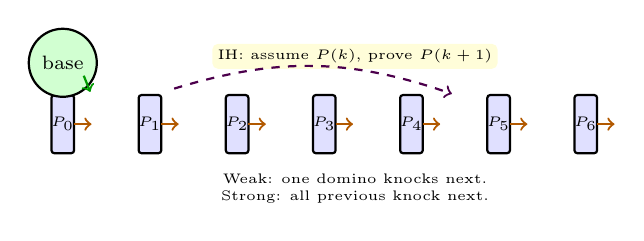
\begin{tikzpicture}[scale=0.82,every node/.style={font=\scriptsize}]
% Domino induction picture
\foreach \i in {0,...,6} {
  \pgfmathsetmacro{\x}{\i*1.35}
  \draw[thick,fill=blue!12,rounded corners=1pt] (\x,0) rectangle++(0.35,0.9);
  \draw[thick,->,orange!70!black] (\x+0.35,0.45)--(\x+0.62,0.45);
  \node[font=\tiny] at (\x+0.175,0.45) {$P_{\i}$};
}
\node[draw,thick,circle,fill=green!18,minimum size=0.6cm] at (0.175,1.4) {base};
\draw[->,thick,green!60!black] (0.5,1.2)--(0.6,0.95);
\node[font=\tiny,fill=yellow!15,rounded corners=2pt,inner sep=2pt] at (4.7,1.5) {IH: assume $P(k)$, prove $P(k+1)$};
\node[font=\tiny,align=center] at (4.7,-0.55) {Weak: one domino knocks next.\\Strong: all previous knock next.};
% strong arrow
\draw[->,thick,violet!60!black,dashed] (1.9,1.0) to[bend left=18] (6.2,0.92);
\end{tikzpicture}
\caption{Induction as dominoes. Weak uses $P(k)$ alone; strong uses $P(n_0),\dots,P(k)$.}
\label{fig:induction-domino}
\end{figure}

\begin{definition}[Weak induction]
To prove $\forall n\ge n_0\,P(n)$: (Base) $P(n_0)$; (Step) $\forall k\ge n_0,\,P(k)\Rightarrow P(k+1)$.
\end{definition}

\begin{theorem}[Sum of first $n$ integers]
$\sum_{i=1}^{n}i=n(n+1)/2$ for $n\ge1$.
\end{theorem}
\begin{proof} Base $1=1\cdot2/2$. IH $\sum_{i=1}^{k}i=k(k+1)/2$. Then $\sum_{i=1}^{k+1}i=k(k+1)/2+(k+1)=(k+1)(k+2)/2$.
\end{proof}

\begin{definition}[Strong induction]
Assume $P(j)$ for all $n_0\le j\le k$ to get $P(k+1)$.
\end{definition}

\begin{theorem}[Every $n\ge2$ has a prime factor]
Every integer $n\ge2$ is divisible by a prime.
\end{theorem}
\begin{proof} Base $2$ prime. Fix $k\ge2$, assume every $2\le j\le k$ has prime divisor. If $k+1$ prime done; else $k+1=ab$ with $2\le a,b\le k$, prime divisor of $a$ divides $k+1$.
\end{proof}

\begin{example}[Faulty induction]
``All horses same colour'': false --- the $P(k)\Rightarrow P(k+1)$ step fails at $k=1$ (overlap needs $\ge2$ horses). Base $n=1$ true, step invalid.
\end{example}

\begin{lstlisting}[language=Python]
# Induction mirrors recursion: prove recursive function correct by induction on n
def fact(n):
    if n==0: return 1          # base P(0)
    return n*fact(n-1)         # step uses P(n-1) to get P(n)

# Strong induction: every n>=2 has prime divisor (constructive)
def prime_divisor(n):
    for p in range(2, n+1):
        if n%p==0 and all(p% d for d in range(2,p)):
            return p
print([prime_divisor(n) for n in range(2,15)])
\end{lstlisting}

\begin{remark}[Choosing weak vs.\ strong]
Use strong when $P(k+1)$ needs not just $P(k)$ but an earlier $P(j)$ (divisors, recurrences with two steps, coin problem). Otherwise weak suffices.
\end{remark}

Every proof begins by unpacking definitions: what does it mean to be even, prime, or divisible?
Direct proof is the workhorse: assume the left, derive the right, step by step.
Contrapositive is useful when the conclusion is a negation, flipping the problem into a positive one.
Contradiction is the tool of impossibility: assume the opposite and find an absurdity.
Induction is the infinite domino chain, turning one base step and one inductive link into all cases.
Strong induction is not stronger logically, just more convenient when the next case needs earlier ones.
Well-ordering, weak induction, and strong induction are three faces of the same principle on $\mathbb{N}$.
A faulty base case can sink an induction, as the horse colour paradox memorably shows.
Loop invariants are just inductions over the number of iterations, connecting MH1812 to algorithm correctness.
Writing the induction hypothesis explicitly prevents the common mistake of assuming what you need to prove.
Every proof begins by unpacking definitions: what does it mean to be even, prime, or divisible?
Direct proof is the workhorse: assume the left, derive the right, step by step.
Contrapositive is useful when the conclusion is a negation, flipping the problem into a positive one.
Contradiction is the tool of impossibility: assume the opposite and find an absurdity.
Induction is the infinite domino chain, turning one base step and one inductive link into all cases.
Strong induction is not stronger logically, just more convenient when the next case needs earlier ones.
Well-ordering, weak induction, and strong induction are three faces of the same principle on $\mathbb{N}$.
A faulty base case can sink an induction, as the horse colour paradox memorably shows.
Loop invariants are just inductions over the number of iterations, connecting MH1812 to algorithm correctness.
Writing the induction hypothesis explicitly prevents the common mistake of assuming what you need to prove.
Every proof begins by unpacking definitions: what does it mean to be even, prime, or divisible?
Direct proof is the workhorse: assume the left, derive the right, step by step.
Contrapositive is useful when the conclusion is a negation, flipping the problem into a positive one.
Contradiction is the tool of impossibility: assume the opposite and find an absurdity.
Induction is the infinite domino chain, turning one base step and one inductive link into all cases.
Strong induction is not stronger logically, just more convenient when the next case needs earlier ones.
Well-ordering, weak induction, and strong induction are three faces of the same principle on $\mathbb{N}$.
A faulty base case can sink an induction, as the horse colour paradox memorably shows.
Loop invariants are just inductions over the number of iterations, connecting MH1812 to algorithm correctness.
Writing the induction hypothesis explicitly prevents the common mistake of assuming what you need to prove.
Every proof begins by unpacking definitions: what does it mean to be even, prime, or divisible?

\begin{theorem}[Well-ordering principle equivalence]
Weak induction, strong induction, and the well-ordering principle (every non-empty $S\subseteq\mathbb{N}$ has a least element) are equivalent.
\end{theorem}
\begin{proof}[Sketch] Well-ordering $\Rightarrow$ strong induction: if $P$ fails, the set $\{n:P(n)\text{ false}\}$ has a least $m$, contradicting $P(j)$ for $j<m\Rightarrow P(m)$. The other directions are exercises.
\end{proof}

\begin{example}[Induction with inequality]
Claim: $2^n>n^2$ for $n\ge5$. Base $32>25$. IH $2^k>k^2$ for $k\ge5$. Then $2^{k+1}=2\cdot2^k>2k^2=k^2+k^2>k^2+2k+1=(k+1)^2$ since $k^2>2k+1$ for $k\ge3$.
\end{example}


\begin{theorem}[Contradiction vs contrapositive]
Contrapositive proves $P\to Q$ by proving $\neg Q\to\neg P$ (one flip). Contradiction assumes $P\land\neg Q$ and derives any absurdity --- strictly more powerful but often overkill.
\end{theorem}

\begin{example}[Irrational $e$ or $\pi$ sketch]
Classical contradictions show $e$ irrational via series remainder $<1/n!$ squeeze; $\pi$ is harder (Lambert).
\end{example}

Direct proof is the workhorse: assume the left, derive the right, step by step.
Contrapositive is useful when the conclusion is a negation, flipping the problem into a positive one.
Contradiction is the tool of impossibility: assume the opposite and find an absurdity.
Induction is the infinite domino chain, turning one base step and one inductive link into all cases.
Strong induction is not stronger logically, just more convenient when the next case needs earlier ones.
Well-ordering, weak induction, and strong induction are three faces of the same principle on $\mathbb{N}$.
A faulty base case can sink an induction, as the horse colour paradox memorably shows.
Loop invariants are just inductions over the number of iterations, connecting MH1812 to algorithm correctness.
Writing the induction hypothesis explicitly prevents the common mistake of assuming what you need to prove.
Every proof begins by unpacking definitions: what does it mean to be even, prime, or divisible?

\subsection{Structural Induction}
\label{sec:structural}
Weak induction climbs numbers; \emph{structural induction} climbs shapes: prove $P$ for every atom (base cases), then show each constructor preserves $P$ (step: $P$ on the parts implies $P$ on the whole built from them). Intuition: recursion builds objects the way induction proves over them---one principle, two directions.
\begin{example}[Full binary trees]
A full binary tree is a leaf, or a node with two full-binary subtrees $L,R$. Claim: $\ell(T)=i(T)+1$ (leaves equal internal nodes plus one). Base: a leaf has $\ell=1,i=0$. Step: $\ell(T)=\ell(L)+\ell(R)=(i(L)+1)+(i(R)+1)=i(T)+1$ since $i(T)=i(L)+i(R)+1$. The step mirrors the constructor exactly.
\end{example}

\section{Worked Example: A Complete Induction Proof Dissected}
Prove $1+3+5+\cdots+(2n-1)=n^2$. Let $P(n)$ be the equality. Base $P(1)$: $1=1^2$. IH $P(k)$: sum to $k$ equals $k^2$. Then sum to $k+1$ is $k^2+(2(k+1)-1)=k^2+2k+1=(k+1)^2$, i.e.\ $P(k+1)$. Every step is explicit: state $P$, check base, assume IH, derive next.

Strong induction example: prove every $n\ge1$ has binary representation. Strong IH: all $j<n$ have binary. If $n$ even, $n=2k$ with $k<n$, take representation of $k$ and append $0$; if $n$ odd, $n=2k+1$, take $k$ and append $1$. Base $1=1_2$. This needs both parities, hence all smaller $j$, not just $n-1$.

% ============================================================
\section{Chapter Notes}
Euclid pioneered indirect proof; induction was formalised by Pascal and Peano. Hoare logic and loop invariants (SC2001) are just induction over iterations. Strong induction $=$ weak induction with strengthened hypothesis $Q(k)=\forall j\le k\,P(j)$.

% ============================================================
\section{Exercises}
\label{sec:ch04-exercises}
\begin{enumerate}[label=E4.\arabic*, leftmargin=*, itemsep=0.6em]
\item \textbf{Direct.} Prove: if $m,n$ even then $m+n$ even; if $a\mid b$ and $a\mid c$ then $a\mid(b+c)$.
\item \textbf{Contrapositive.} Prove: if $n^2$ divisible by $3$ then $n$ divisible by $3$. Why is direct messy? Write the contrapositive explicitly.
\item \textbf{Contradiction.} Prove $\sqrt3$ irrational and that there is no smallest positive rational (if $r>0$ rational then $r/2$ smaller positive rational --- contradiction to minimality).
\item \textbf{Induction.} Prove $\sum_{i=1}^{n}i^2=n(n+1)(2n+1)/6$ and $2^n>n$ for $n\ge1$ by weak induction.
\item \textbf{Strong induction.} Every $n\ge12$ is $4a+5b$ for $a,b\ge0$. Prove by strong induction with bases $12,13,14,15$. Where does weak fail?
\end{enumerate}
% End of Chapter 4
